\subsection{Examining the Starter Code}

\paragraph{user\_controls.c}
The \function{initialize_controls()} function is where you'll place any alarm-related code that needs to be run once when the program starts.
The \function{manage_controls()} function is where you'll place any alarm-related code that needs to run with every iteration of the program's main loop.
You may, of course, add helper functions.

\paragraph{shared\_variables.h}
This is the only header file you will turn in, so if you need to share any \lstinline{enum}s, \lstinline{struct}s, or variables between \textit{.c} files, place them in here and not in the other header files, so that we can compile your code.
When you need to share a variable between \textit{.c} files, declare it in exactly one \textit{.c} file (preferably the one that the variable best coheres to) without the \lstinline{extern} keyword,
and then externalize it by declaring it again with the \lstinline{extern} keyword in \textit{shared\_variables.h}.
This approach will create just one global symbol for the variable in the program while making it ``visible'' to the code in the other \textit{.c} files.

\subsection{A Quick Note about Creating State Machines}

A not-uncommon pattern in embedded systems is to design the system as a state machine, or as multiple state machines.
The states are represented as the value of an enumerated type.
A couple of key advantages of writing the system as a state machine or as a collection of state machines is that it's easy to change the state based on inputs,
and it's easy for the parts of the system that take action to do so based on what state the state machine is in.

\subsection{Read the Switches}

\begin{figure}[h]
    \centering
    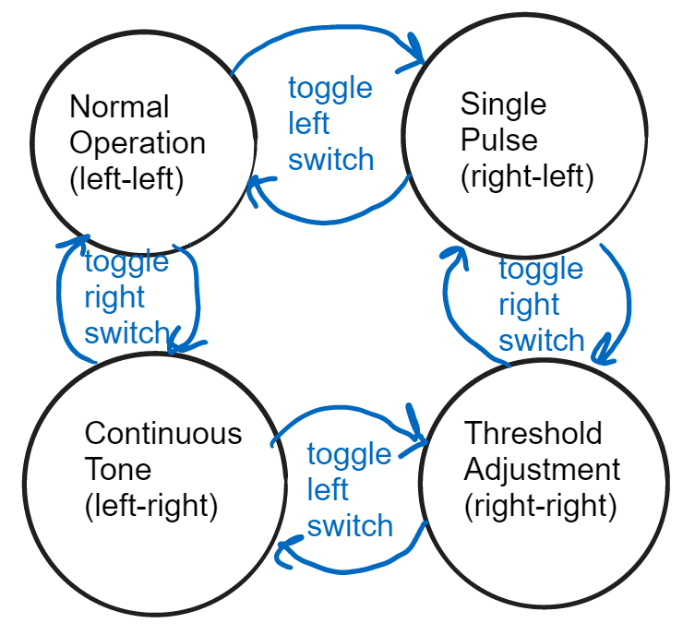
\includegraphics[width=3in]{modeStateMachine}
    \caption{\label{fig:modeStateMachine} State machine describing the rangefinder's modes of operation.}
\end{figure}

Create a way to track which mode the system is in (Requirement~\ref{spec:modes}).
Be sure to declare it not only in \textit{user\_controls.c} (without the \lstinline{extern} modifier) but also in \textit{shared\_variables.h} (with the \lstinline{extern} modifier).
Add code to \function{manage_controls()} to poll the positions of the slide-switches and set the system's mode accordingly.

\subsection{Read the Pushbutton} \label{subsec:readPushbutton}

As noted in Requirement~\ref{spec:singlePulseOperation}, if the system is in Single-Pulse Operation mode and the user presses the left pushbutton, they want to emit exactly one ultrasound pulse to get the distance to an object.
\begin{figure}[h]
    \centering
    \includegraphics[width=10cm]{internet_images/one_ping_only}
    \caption{Verify our range to target. One ping only. \\ \tiny Image by Paramount Pictures Corporation \label{fig:onePingOnly}}
\end{figure}

Create a variable to indicate that the user has requested a ping.
Be sure to declare it not only in \textit{user\_controls.c} (without the \lstinline{extern} modifier) but also in \textit{shared\_variables.h} (with the \lstinline{extern} modifier).
Add code to \function{initialize_controls()} to set this variable initially to \lstinline{false}.
Add code to \function{manage_controls()} to set this variable to \lstinline{true} when and only when the use presses the button while in Single-Pulse Operation mode.
The variable should be set to \lstinline{true} only \textit{once} per press.
(Do \textit{not} set it to \lstinline{true} just because the user is still holding the button down.)

Do not worry about setting this variable to \lstinline{false} yet;
that will come later.

\vspace{1cm}

You can now continue to work through the remainder of the lab with your partner, perhaps pair programming,
or you can decide to have one partner work on Section~\ref{sec:distance} and the other work on Section~\ref{sec:sound}.
Regardless, you will need to work together on Section~\ref{sec:integration}, as this is when you will integrate the work from Sections~\ref{sec:distance}--\ref{sec:sound}.
